%%==================================================
%% chapter04.tex for BIT Master Thesis
%% modified by 朱杰
%%==================================================
\chapter{基于稳定标签传播的重叠社区发现算法}
在验证了上一章所提稳定策略在 LPA 算法上的有效性的基础上,将此稳定策略运用到 COPRA 算法中,以验证其在重叠社区发现算法中的有效性。

本章提出一种基于稳定标签传播的重叠社区发现算法(Overlapping Community Detection Algorithm Based on Stable Label Propagation),下文简称 OCDABSLP。OCDABSLP 算法在迭代执行标签更新过程中,当节点属于所有社区的隶属度都小于阈值且最大值有多个时,选择隶属度最大的多个标签中标签影响强度最大的标签。满足终止条件后,算法根据节点的标签将其划分到相应社区中,拥有多个标签的节点被划分到相应的多个社区中,成为重叠节点,得到最终的重叠社区划分结果。在不同复杂网络数据集上的大量实验表明本章算法能够得到比现有的大部分算法更好的社区划分结果。

\section{多标签传播算法(COPRA)}

Gregory 等人[40]提出的 COPRA 算法是第一个利用标签传播思想进行重叠社
区发现的算法。算法中每个节点可以以不同隶属度拥有多个标签,每个节点包含
一组标签-隶属度对$(l, b)$,$l $表示节点所属社区的编号,$b $表示节点属于该社区的
隶属程度,$b_t(l, i)$表示在第$ t $次标签传播结束时节点$ i $属于社区$ l $的隶属程度。
COPRA 通过迭代地更新各个节点的标签及隶属度来获取社区结构。

与 LPA 算法相同,初始时,COPAR 算法为每个节点分配一个各不相同的标
签,并将其隶属度设置为 1,即 $b_0(i, i) = 1$。然后采用同步更新策略进行标签更新
迭代,在每次更新过程中,用邻接点中出现的所有相同标签的平均隶属度更新该
节点的标签-隶属度对列表。每一轮更新后,删除隶属度小于 $\frac{1}{v}$ 的标签($v$ 是算法的参数),当一个节点的所有标签对应的隶属度都小于 $\frac{1}{v}$ 时,就只保留一个
隶属度最大的标签,若此时有多个标签的隶属度同时取最大值,就随机保留隶属
度最大的标签中的一个,然后对所有剩余标签的隶属度进行归一化。更新结束后,
算法根据节点的标签将其划分到相应的社区中。一个节点最后拥有的标签数即为
它被划分到的社区的个数。 

函数 $b_t(l, i)$用于计算在第 $t $次迭代中,节点$ i $属于社区$ l $的隶属程度,计算如
公式\ref{eqn:lishudu}所示。

\begin{equation}
  \label{eqn:lishudu}
  b_t(l,i)=\frac{\sum_{j\in \Gamma_i }b_{t-1}(l,j)}{d_i}
\end{equation}

COPRA 算法的执行过程如算法 所示。

算法:多标签传播算法(COPRA) 

输入:复杂网络 $G = (V, E)$,最大迭代次数 $maxRun$ 

输出:社区划分结果 

Step1:  初始化,为网络中的每个节点分配一个各不相同的标签,标签-隶属度对集合为${(i,l)}$;令迭代次数$t=0$。

Step2:  标签传播迭代过程 

(a)如果迭代次数 $t > maxRun$,标签传播迭代过程结束,转 Step3;否则继续算法。 

(b)对于每个节点$v_i\in V$,根据公式\ref{eqn:lishudu}计算该节点属于其邻接点集合中出现的所有标签的隶属度,更新标签-隶属度对列表。根据参数$v$删除不满足条件的标签,并对剩余标签进行归一化。 
 
(c)如果连续两次迭代结束后,标签集合的大小不变,那么标签传播迭代过程停止,
转Step3;否则,令$t = t+1$转到步骤(a)继续执行。 

Step3:  社区划分,将拥有相同标签的节点划分到同一个社区中,不同标签的种类就表示网络中社区的个数。

COPRA 算法继承了 LPA 算法的优点,也保留了 LPA 算法稳定性和鲁棒性差等缺点。 

\section{算法设计}
原始COPRA算法中的唯一一个不稳定因素是当节点属于所有社区的隶属度
都小于阈值且最大值有多个时,会随机选择一个标签。因此,在此处对 COPRA
算法进行改进。当出现上述情形时,选择隶属度最大的多个标签中标签影响强度
最大的标签。当标签影响强度最大的标签仍有多个时,保留所有标签影响强度最
大的标签。标签影响强度的计算如公式\ref{eqn:LI2}所示。

\begin{equation}
  \label{eqn:LI2}
  NI(i,l)=\sum_{j \in \Gamma _i} b_{t-1}(l,j) \frac{NI(j)}{d_j}
\end{equation}

OCDABSLP 算法的主要步骤包括初始化、迭代标签传播和社区划分。图\ref{fig:fig4-1}
为 OCDABSLP 的算法流程图。

\begin{figure}
  \centering
  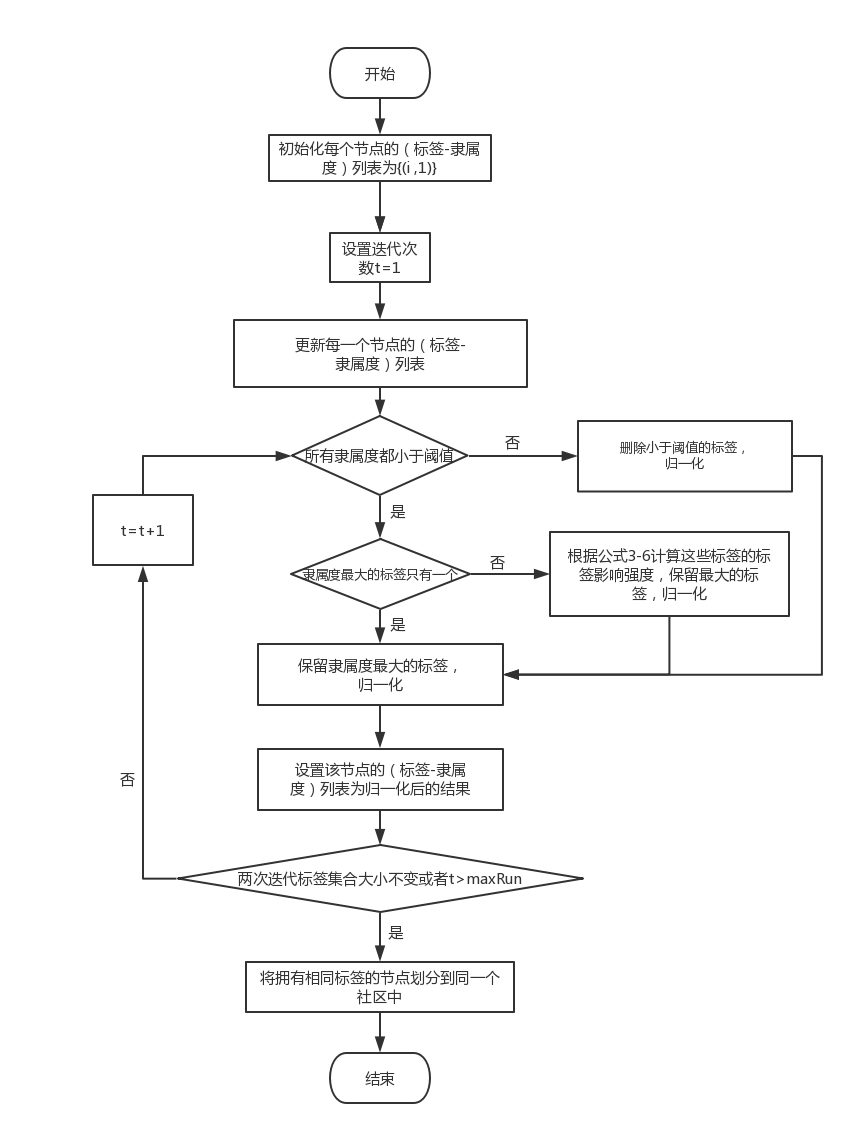
\includegraphics[width=1\textwidth]{figures/fig4-1}
  \caption{OCDABSLP算法流程图}\label{fig:fig4-1}
\end{figure}

\section{算法时间复杂度分析}
OCDABSLP 算法的时间复杂度分析如下: 

(1)为每个节点初始化标签所用时间复杂度为$ O(|V|)$; 

(2)每次标签传播过程分为两部分: 传统的标签传播过程:$O(v|E|log(v|E|/|V|))$;当节点属于所有社区的隶属度都小于阈值且最大值有多个时,利用
公式\ref{eqn:LI2}计算标签影响值的过程:$O(v|E|log(v|E|/|V|))$; 

(3)将相同标签的节点划分到一个社区的时间复杂度为 $O(|V|)$。 

标签传播过程是不断迭代执行的,因此整个算法的时间复杂度为
$2O(|V|)+2tO(v|E|log(v|E|/|V|))$。

\section{算法伪代码}